\documentclass[12pt]{article}
\usepackage{amsmath}
\usepackage{array}
\usepackage{gensymb}
\usepackage{geometry}
\usepackage{graphicx}
\usepackage{pgfplots}
\usepackage{siunitx}
\usepackage{wrapfig}

\title{Homework \#3}
\author{Donald Aingworth IV}
\date{September 11, 2024}

\pgfplotsset{width=8cm,compat=1.9}
\usepgfplotslibrary{external}
% \tikzexternalize

\begin{document}

\DeclareSIUnit{\mile}{mi}
\DeclareSIUnit{\gal}{gal}
\DeclareSIUnit{\foot}{ft}
\DeclareSIUnit{\h}{h}

\maketitle

\section*{Problem 1}
Is it possible to have $|\Vec{A} + \Vec{B}|$ = $|\Vec{A} - \Vec{B}|$ = ? If so, illustrate with a diagram.

\subsection*{Solution}
We can use the law of cosines as the formula for the magnitude of a sum or two vectors. Assume that $\theta$ is the angle between the two vectors.

\begin{align*}
    |\Vec{A} + \Vec{B}| &= |\Vec{A} - \Vec{B}|\\
    \sqrt{|\Vec{A}|^2 + |\Vec{B}|^2 - 2\Vec{A}\Vec{B}\cos(\theta)} &= \sqrt{|\Vec{A}|^2 + |\Vec{B}|^2 - 2\Vec{A}(-\Vec{B})\cos(\theta)}\\
    |\Vec{A}|^2 + |\Vec{B}|^2 - 2\Vec{A}\Vec{B}\cos(\theta) &= |\Vec{A}|^2 + |\Vec{B}|^2 + 2\Vec{A}\Vec{B}\cos(\theta)\\
    - 2\Vec{A}\Vec{B}\cos(\theta) &= 2\Vec{A}\Vec{B}\cos(\theta)\\
    -\cos(\theta) &= \cos(\theta)\\
    2\cos(\theta) &= 0\\
    \cos(\theta) &= 0\\
    \theta &= \pm \frac{\pi}{2}
\end{align*}

As such, it is possible to have $|\Vec{A} + \Vec{B}|$ = $|\Vec{A} - \Vec{B}|$. This is the instance where $\Vec{A}$ and $\Vec{B}$ are perpendicular. 

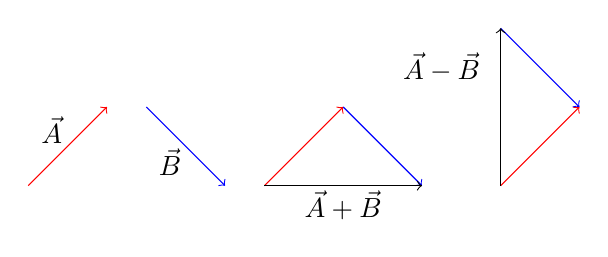
\begin{tikzpicture}
    \draw [ red,thin,-> ] (0,0) -- (1,1); \node at (0.3,0.7) {$\Vec{A}$};
    \draw [ blue,thin,-> ] (1.5,1) -- (2.5,0); \node at (1.8,0.3) {$\Vec{B}$};
    
    \draw [ red,thin,-> ] (3,0) -- (4,1);
    \draw [ blue,thin,-> ] (4,1) -- (5,0);
    \draw [ black,thin,-> ] (3,0) -- (5,0); \node at (4,-0.25) {$\Vec{A} + \Vec{B}$};

    \draw [ red,thin,-> ] (6,0) -- (7,1);
    \draw [ blue,thin,-> ] (6,2) -- (7,1);
    \draw [ black,thin,-> ] (6,0) -- (6,2); \node at (5.25,1.5) {$\Vec{A} - \Vec{B}$};
\end{tikzpicture}

Above is the diagram. Using vector coordinates and the magnitude formula, we will find that the magnitudes of $|\Vec{A} + \Vec{B}|$ and $|\Vec{A} - \Vec{B}|$ are equivalent.

\pagebreak
\section*{Problem 2}
Four vectors, each of magnitude 2.50 m, are shown in the figure. (a) Express each in unit
vector notation. (b) Express their sum in unit vector notation. (c) What is the magnitude and direction of their sum?

\begin{center}
    \includegraphics*[width=10cm]{graph_2.png}
\end{center}

\subsection*{Solution}

a) Name the vectors $v_A,\ v_B,\ v_C, \text{ and } v_D$. $v_A$ is clockwise from the +x axis, so we replace the angle with 360$\degree$ minus the angle. $v_B$ is clockwise from the +y axis, so we replace the angle with 90$\degree$ minus the angle. $v_C$ is counterclockwise from the +x axis, so we take it at its angle apparent. $v_D$ is clockwise from the +x axis, so we replace the angle with 360$\degree$ minus the angle. We then put the answers to the overall vector in the final column of the below table of vectors and calculations.
\begin{center}
    \begin{tabular}{ c | c | c | c | c }
        v & (r, axis - $\theta_0$) & (r, $\theta$) & $r\cos(\theta)\hat{i}+r\sin(\theta)\hat{j}$ & $v_x\hat{i} + v_y\hat{j}$\\ \hline
        $v_A$ & $(\frac{5}{2}, 360\degree - 120\degree)$ & $(\frac{5}{2}, 240\degree)$ & $\frac{5}{2}\cos(240\degree)\hat{i} + \frac{5}{2}\sin(240\degree)\hat{j}$ & $-\frac{5}{4}\hat{i} -\frac{5\sqrt{3}}{4}\hat{j}$\\
        $v_B$ & $(\frac{5}{2}, 90\degree - 50\degree)$ & $(\frac{5}{2}, 40\degree)$ & $\frac{5}{2}\cos(40\degree)\hat{i} + \frac{5}{2}\sin(40\degree)\hat{j}$ & $1.915\hat{i} + 1.607\hat{j}$\\
        $v_C$ & $(\frac{5}{2}, 0\degree + 150\degree)$ & $(\frac{5}{2}, 150\degree)$ & $\frac{5}{2}\cos(150\degree)\hat{i} + \frac{5}{2}\sin(150\degree)\hat{j}$ & $-\frac{5\sqrt{3}}{4}\hat{i} + \frac{5}{4}\hat{j}$\\
        $v_D$ & $(\frac{5}{2}, 360\degree - 35\degree)$ & $(\frac{5}{2}, 325\degree)$ & $\frac{5}{2}\cos(325\degree)\hat{i} + \frac{5}{2}\sin(325\degree)\hat{j}$ & $2.047\hat{i} -1.434\hat{j}$\\
    \end{tabular}
\end{center}

\pagebreak
b) $0.548\hat{i} - 0.742\hat{j}$
\begin{align*}
    v_A+v_B+v_C+v_D =   &(-\frac{5}{4} + 1.915 - \frac{5\sqrt{3}}{4} + 2.047)\hat{i}\\
                        &+ (-\frac{5\sqrt{3}}{4} + 1.607 + \frac{5}{4} - 1.434)\hat{j}\\
                    =   &\boxed{0.548\hat{i} - 0.742\hat{j}}
\end{align*}

c) (r, $\theta$) = (0.922, $-53.6\degree$) or (0.922, $306.4\degree$)

For the magnitude, we merely use the pythagorean theorem on the above vector.
\begin{align*}
    \sqrt{x^2 + y^2}    &= \sqrt{0.548^2 + 0.742^2}\\
                        &= \sqrt{0.300 + 0.551}\\
                        &= \sqrt{0.851}\\
                        &= \boxed{0.922}
\end{align*}

For the direction, we can find the arctangent to the vector's slope.
\begin{equation*}
    \theta = \arctan \left( \frac{v_y}{v_x} \right) = \arctan \left( \frac{-0.742}{0.548} \right) \approx \boxed{-53.6\degree}
\end{equation*}
That angle is equivalent to $306.4\degree$.


\pagebreak
\section*{Problem 3}
An object follows as shown below. What is the displacement from the last point to the
starting point? Express your answer (a) in unit vector notation, and (b) as a magnitude and direction.

\begin{center}
    \includegraphics*[width=10cm]{graph_3.png}
\end{center}

\subsection*{Solution}
a) $\frac{7\sqrt{2}}{4}\hat{i} + \frac{\sqrt{2}}{4}\hat{j}$

Name the vectors $v_1,\ v_2, \text{ and } v_3$. We then put the values of the overall vector in the final column of the below table of vectors and calculations.
\begin{center}
    \begin{tabular}{ c | c | c | c }
        v & (r, original - $\theta_0$) & $r\cos(\theta)\hat{i}+r\sin(\theta)\hat{j}$ & $v_x\hat{i} + v_y\hat{j}$\\ \hline
        $v_1$ & $(2\unit{\km},0\degree + 45\degree)$ & $2\cos(45\degree)\hat{i} + 2\sin(45\degree)\hat{j}$ & $\sqrt{2}\ \hat{i}\unit{km} + \sqrt{2}\ \hat{j}\unit{km}$\\
        $v_2$ & $(\frac{3}{2}\unit{\km},45\degree - 30\degree)$ & $\frac{3}{2}\cos(15\degree)\hat{i} + \frac{3}{2}\sin(15\degree)\hat{j}$ & $\frac{3\sqrt{2}(\sqrt{3}+1)}{8}\hat{i}\unit{km} + \frac{3\sqrt{2}(\sqrt{3}-1)}{8}\hat{j}\unit{km}$\\
        $v_3$ & $(\frac{3}{2}\unit{\km},15\degree - 120\degree)$ & \small$\frac{3}{2}\cos(255\degree)\hat{i} + \frac{3}{2}\sin(255\degree)\hat{j}$ & $\frac{3\sqrt{2}(\sqrt{3}-1)}{8}\hat{i}\unit{km} + \frac{3\sqrt{2}(\sqrt{3}+1)}{8}\hat{j}\unit{km}$
    \end{tabular}
\end{center}

We then add the four together.
\[
    v_1 + v_2 + v_3 = (\sqrt{2} + \frac{3}{4}\sqrt{2})\hat{i} + (\sqrt{2} - \frac{3}{4}\sqrt{2})\hat{j} = \boxed{\frac{7\sqrt{2}}{4}\hat{i} + \frac{\sqrt{2}}{4}\hat{j}}
\]

\pagebreak
b) $(\frac{5}{2},188.13\degree)$

For the magnitude, we merely use the pythagorean theorem on the above vector.
\[
    \sqrt{x^2 + y^2} = \sqrt{\frac{7\sqrt{2}}{4}^2 + \frac{\sqrt{2}}{4}^2} 
                    = \sqrt{\frac{49}{8} + \frac{1}{8}} 
                    = \sqrt{\frac{50}{8}} 
                    = \sqrt{\frac{25}{4}} 
                    = \boxed{\frac{5}{2}}
\]

For the direction, we can find the arctangent to the vector's slope.
\begin{equation*}
    \theta = \arctan \left( \frac{v_y}{v_x} \right) = \arctan \left( \frac{1}{7} \right) \approx 8.13\degree
\end{equation*}

Since we are looking for the displacement back to the starting point, we add $180\degree$ to this to get \boxed{188.13\degree}

\pagebreak
\section*{Problem 4}
Given two vectors, $\Vec{A}$ = 5.00 $\hat{i}$ + 2.00 $\hat{j}$, and $\Vec{B}$ = -2.00 $\hat{i}$ - 3.00 $\hat{j}$, find (a) $\Vec{A}$ + $\Vec{B}$ ; (b) $\Vec{A}$ + $\Vec{B}$; (c) $|\Vec{A}$ - $\Vec{B}|$ (d) $\Vec{A}$ - $\Vec{B}$.

\subsection*{Solution}

a) $3\hat{i} - 1\hat{j}$
\begin{equation*}
    \Vec{A} - \Vec{B} = 5\hat{i} + 2\hat{j} - 2\hat{i} - 3\hat{j} = 3\hat{i} - 1\hat{j}
\end{equation*}
b) $\sqrt{10}$
\begin{equation*}
    \sqrt{x^2+y^2} = \sqrt{3^2+1^2} = \sqrt{9+1} = \sqrt{10}
\end{equation*}
c) $7\hat{i} + 5\hat{j}$
\begin{equation*}
    \Vec{A} + \Vec{B} = 5\hat{i} + 2\hat{j} + 2\hat{i} + 3\hat{j} = 7\hat{i} + 5\hat{j}
\end{equation*}
d) $\sqrt{74}$
\begin{equation*}
    \sqrt{x^2+y^2} = \sqrt{7^2+5^2} = \sqrt{49+25} = \sqrt{74}
\end{equation*}


\pagebreak
\section*{Problem 5}
Find the components of the following vectors: (a) P of length 5.50 m directed at $160\degree$ counterclockwise from the +x axis; (b) Q of length 3.50 m directed at $120\degree$ clockwise from the +y axis.

\subsection*{Solution}

\begin{center}
    \begin{tabular}{ c | c | c | c }
        v & (r, original - $\theta_0$) & $r\cos(\theta)\hat{i}+r\sin(\theta)\hat{j}$ & $v_x\hat{i} + v_y\hat{j}$ (Solution)\\ \hline
        (a) & $(\frac{11}{2}\unit{\m},0\degree + 160\degree)$ & $\frac{11}{2}\cos(160\degree)\hat{i} + \frac{11}{2}\sin(160\degree)\hat{j}$ & $-5.168 \hat{i}\unit{m} + 1.881 \hat{j}\unit{m}$\\
        (b) & $(\frac{7}{2}\unit{\m},450\degree - 120\degree)$ & $\frac{7}{2}\cos(330\degree)\hat{i} + \frac{7}{2}\sin(330\degree)\hat{j}$ & $\frac{7\sqrt{3}}{4}\hat{i}\unit{m} - \frac{7}{4}\hat{j}\unit{m}$
    \end{tabular}
\end{center}

\pagebreak
\section*{Problem 6}
Two vectors have equal magnitudes of 2.0 m. Find graphically the angle between them if the magnitude of their resultant is (a) 3.0 m; (b) 1.0 m. In each case use the law of cosines to confirm your answer.

\subsection*{Solution}

Here, we can manipulate the law of cosines to isolate cos($\theta$).
\begin{eqnarray*}
    c^2 = a^2 + b^2 - 2ab\cos(\theta)\\
    2ab\cos(\theta) = a^2 + b^2 - c^2\\
    \cos(\theta) = \frac{a^2 + b^2 - c^2}{2ab}
\end{eqnarray*}

a) $82.8\degree$\\
For a=b=2m and c=3m.
\begin{align*}
    \cos(\theta) &= \frac{a^2 + b^2 - c^2}{2ab} = \frac{2^2 + 2^2 - 3^2}{2*2*2}\\
                 &= \frac{4+4-9}{8} = -\frac{1}{8}\\
    \theta &= \boxed{ \cos\left(-\frac{1}{8}\right) \approx 97.2\degree }
\end{align*}

Since we now have the intersecting angle of the triangle the two make when added together, the angle between the two is the complement of that angle. We subtract 180 degrees from the angle we found to get: $180\degree - 97.2\degree = \boxed{82.8\degree}$.
\pagebreak

b) $151.0\degree$\\
For a=b=2m and c=1m.
\begin{align*}
    \cos(\theta) &= \frac{a^2 + b^2 - c^2}{2ab} = \frac{2^2 + 2^2 - 1^2}{2*2*2}\\
                 &= \frac{4+4-1}{8} = \frac{7}{8}\\
    \theta &= \boxed{ \cos\left(\frac{7}{8}\right) \approx 29.0\degree }
\end{align*}

Since we now have the intersecting angle of the triangle the two make when added together, the angle between the two is the complement of that angle. We subtract 180 degrees from the angle we found to get: $180\degree - 29.0\degree = \boxed{151.0\degree}$.

\pagebreak
\section*{Problem 7}
An airplane is flown in the direction 30$\degree$ W of N. If the magnitude of the westerly component of the displacement is 100 km, how far north does it travel?

\subsection*{Solution}

Thirty degrees West of North would be 120 degrees counterclockwise of East. If we multiply the western distance (-100 since West is in the negative direction) by the tangent ($\frac{opposite}{adjacent}=\frac{North}{West}$) of the angle, we will get the distance it traveled North.
\[
    -100*\tan(120\degree) = \boxed{100\sqrt{3} \approx 173\unit{km}}
\]

\pagebreak
\section*{Problem 8}
A rectangular coordinate system with axes x' and y' is rotated by angle $\theta$ from axes x and y as shown in the figure. (a) What are the components of the position vector r in the two coordinate systems? (b) Use the results of part (a) to shown that the coordinates of a point P in the two systems are related by
\begin{align*}
    x' &= x \cos(\theta) + y \sin(\theta)\\
    y' &= -x \sin(\theta) + y \cos(\theta)
\end{align*}

\textit{Hint, it might help to expand $\cos(\phi - \theta)$ and $\sin(\phi - \theta)$.}

\begin{center}
    \includegraphics*[width=10cm]{graph_8.png}
\end{center}

\subsection*{Solution}

a) The components of \textbf{r} are those for any vector given the magnitude-angle formula.
\begin{eqnarray*}
    \boxed{\Vec{r}_{xy} = x\hat{i} + y\hat{j} = |r|\cos(\phi)\hat{i} + |r|\sin(\phi)\hat{j}}
\end{eqnarray*}

In the x'y' plane, we only have to replace $\theta$ with $\phi-\theta$.
\begin{eqnarray*}
    \boxed{\Vec{r}_{x'y'} = x'\hat{i} + y'\hat{j} = |r|\cos(\phi-\theta)\hat{i} + |r|\sin(\phi-\theta)\hat{j}}
\end{eqnarray*}
\pagebreak

b) First, we expand $\Vec{r}_{x'y'}$.
\begin{align*}
    \Vec{r}_{x'y'} =\ &|r|\cos(\phi-\theta)\hat{i} + |r|\sin(\phi-\theta)\hat{j}\\
                    =\ &(|r|\cos(\phi)\cos(\theta) + |r|\sin(\phi)\sin(\theta))\hat{i}\\ 
                    &+ (|r|\sin(\phi)\cos(\theta) - |r|\cos(\phi)\sin(\theta))\hat{j}
\end{align*}

Then, we can look over and isolate terms in $\Vec{r}_{x'y'}$ and like terms we can replace in them from $\Vec{r}_{xy}$.
\begin{align*}
    \Vec{r}_{xy} &= |r|\cos(\phi)\hat{i} + |r|\sin(\phi)\hat{j}\\
    x' &= |r|\cos(\phi)\cos(\theta) + |r|\sin(\phi)\sin(\theta) &x = |r|\cos(\phi)\\
    y' &= |r|\sin(\phi)\cos(\theta) - |r|\cos(\phi)\sin(\theta) &y = |r|\sin(\phi)
\end{align*}

We can then replace the terms.
\begin{align*}
    \boxed{x' = x\cos(\theta) + y\sin(\theta)}\\
    \boxed{y' = y\cos(\theta) - x\sin(\theta)}
\end{align*}

\end{document}